\begin{figure*}[tb]
	\centering
	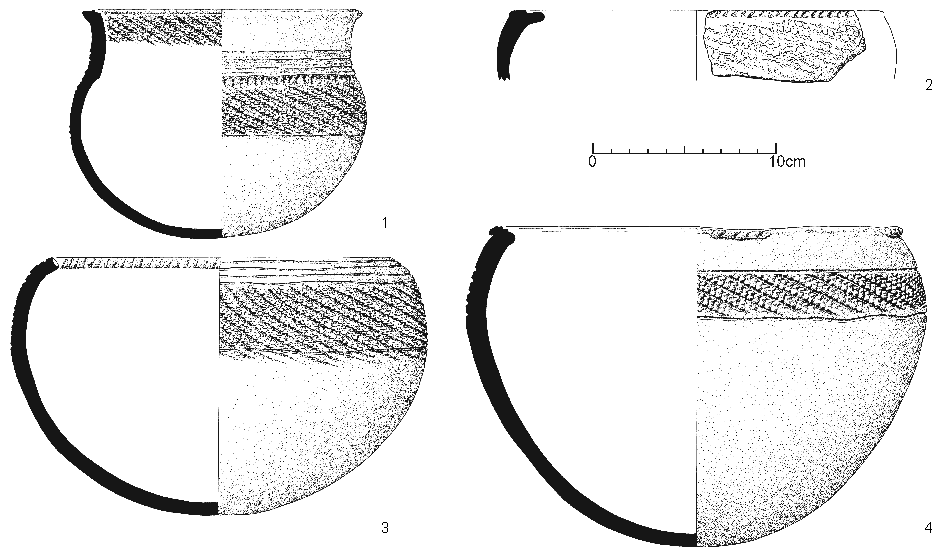
\includegraphics[width=\textwidth]{fig/MBN-Typen.pdf}
	\caption{Mbati-Ngombe-Gruppe: Typvertreter.\\1:~Taf.~10.10; 2:~Taf.~27.11; 3:~Taf.~10.9; 4:~Taf.~10.11.}
	\label{fig:MBN_Typvertreter}
\end{figure*}

\subsubsection{Mbati-Ngombe-Gruppe}\label{sec:MBN-Gr}

Die Mbati-Ngombe-Gruppe beschreibt eine rezente, vegetabilische Roulettes verwendende Keramik, die vor allem am mittleren \mbox{Ubangi} sowie am prospektierten Teil des Lua zu finden ist (Abb.~\ref{fig:MBN_Verbreitung}). Am eponymen Fundort am mittleren \mbox{Ubangi} (Fpl.~204) wurde die Herstellung mehrerer Gefäße beobachtet und dokumentiert.\footnote{Siehe Anm.~\ref{ftn:EthnoToepfereiInVorb}.} Insgesamt vier Gefäße wurden angekauft (Abb.~\ref{fig:MBN_Typvertreter}.1,3--4). Die Stilgruppe umfasst 24~GE aus 14 unterschiedlichen Fundstellen. Keine der Mbati-Ngombe-Gruppe zurechenbare GE stammt aus einer Grabung. Das Material wurde sämtlich von rezenten Dorfflächen abgesammelt oder als \textit{Ethnographica} angekauft. Bestimmende Charakteristika der Inventare sind flache Gefäße mit geschweifter Wandung (Abb.~\ref{fig:MBN_Typvertreter}.1), wie sie auch in der ebenfalls rezenten Dama-Gruppe vorkommen (Kap.~\ref{sec:DAM-Gr}) und schalenförmige Gefäße mit konvexer Wandung und einbiegendem Rand (Abb.~\ref{fig:MBN_Typvertreter}.2--4), wie sie von der Kpetene-Gruppe bekannt sind (Kap.~\ref{sec:KPT-Gr}), sowie eine Verzierungspraxis, die sich lediglich durch die Nutzung vegetabilischer Roulettes von der der Dama-Keramik unterscheidet. Die Beschreibung der Mbati-Gombe-Gruppe basiert vornehmlich auf sechs kompletten Gefäßen (25\,\%) und einer Reihe von Randstücken (58\,\%). 


\paragraph{Technologische Merkmale}\hspace{-.5em}|\hspace{.5em}%
Aus technischer Sicht entsprechen die GE der Mbati-Ngombe-Gruppe den zeitgleichen keramischen Inventaren am mittleren und oberen \mbox{Ubangi}. Die Scherben enthalten fast ausschließlich hohe Anteile heterogener Quarzsande (74\,\%) und nur selten Schamott oder rötliche Partikel, bei denen es sich um zerstoßenen Laterit handeln könnte. Die Partikel gehören größtenteils der Größenklasse \textit{coarse} an (65\,\%), während kleinere (\textit{medium}) sowie größere Korngrößen (\textit{very coarse}) in gleichem Maße vorkommen (je 17\,\%). Bei den \textit{Fabrics} zeigt sich eine gewisse Heterogenität, da die Typen 3c, 4c und 5a zu gleichen Anteilen beobachtet wurden (je 17\,\%). Nur etwas seltener konnte das \textit{Fabric} 4a beobachtet werden (13\,\%). Zudem zeigen nur wenige der Stücke (13\,\%) die Nutzung weißbrennender Tone an, während sich das Gros (48\,\%) aufgrund grauer, beiger oder schwarzer Färbung nicht näher ansprechen lässt. Eine nicht unerhebliche Zahl der GE weist jedoch auf die Nutzung rotbrennender Tone hindeutende Färbungen auf (40\,\%). Die Oberflächen der meisten Scherben sind glatt (70\,\%) oder nur leicht rau (26\,\%).

\begin{figure*}[p]
	\centering
	\includegraphics[width=\textwidth]{fig/MBN_Verbreitung.pdf}
	\caption{Mbati-Ngombe-Gruppe: Verbreitung.}
	\label{fig:MBN_Verbreitung}
\end{figure*}

\paragraph{Formen}\hspace{-.5em}|\hspace{.5em}%
Im Fall von 19~GE war eine Ansprache der Gefäßform möglich. Aufgrund der Fragmentierung der Stücke aus den Oberflächenabsammlungen war nur bei etwas über der Hälfte eine sichere Bestimmung möglich. Zu gleichen Anteilen finden sich flache Gefäße mit geschweifter Wandung und ausgeprägtem Gefäßhals (Typ E; 37\,\%) und schalenförmige Gefäße mit konvexer Wandung und einbiegendem Rand (Typ H; 37\,\%; Abb.~\ref{fig:MBN_Typvertreter}.2--4). Innerhalb der flachen Gefäße mit geschweifter Wandung findet sich vornehmlich der Typ E2 (24\,\%; Abb.~\ref{fig:MBN_Typvertreter}.1). Lediglich eine GE war als Flasche ansprechbar (Typ A; 5\,\%). Die Randgestaltung der Mbati-Ngombe-Gefäße ist, ähnlich wie im Fall der Dama-Gruppe (Kap.~\ref{sec:DAM-Gr}) sehr variabel. Die Randabschlüsse sind vornehmlich rund ausgeformt (M1; 47\,\%). Seltener fanden sich spitze (M2; 16\,\%) oder gerillte Randlippen (M4; 10\,\%). Die häufigste Randform sind konvex einbiegende Ränder (C3; 37\,\%; Abb.~\ref{fig:MBN_Typvertreter}.3), die sich auschließlich an schalenförmigen Gefäßen mit konvexer Wandung (H) finden. Daneben kommen konkav ausbiegende Ränder (B2; 16\,\%; Abb.~\ref{fig:MBN_Typvertreter}.1), einfach ausbiegende (B1; 11\,\%), umgelegte (A2; 11\,\%) sowie einfach einbiegende Ränder vor (C1; 11\,\%). Die flachen Gefäße mit geschweifter Wandung weisen durchweg konkav ausgearbeitete oder zylindrische Hälse auf. Die Schulterbereiche der Gefäße, die eine ausgearbeitete Schulter aufweisen, sind fast ausschließlich konvex (75\,\%) oder gerade (12\,\%) ausgeformt. Nur eine GE zeigt einen Schulterabsatz. Die Gefäßkörper sind mit Ausnahme einer GE deutlich konvex ausgeformt (93\,\%). Bei fünf GE war es möglich, einen runden Gefäßboden zu identifizieren. Eine Ausnahme bildet eine GE vom eponymen Fundplatz Mbati-Ngombe (Fpl.~204), die einen Flachboden mit konkaver Standfläche aufwies (Taf.~10.12).


\paragraph{Verzierungen}\hspace{-.5em}|\hspace{.5em}%
Die Verzierungspraxis der Mbati-Ngombe-Keramik setzt sich vornehmlich aus drei Gruppen von Verzierungselementen zusammen (Anlage~4.10): vegetabilisches \mbox{Roulette} (Tab.~\ref{tab:Verzierungselemente}: 21.1--3), vor allem auf der Innenseite der Ränder sowie im Schulter- und Bauchbereich, die zusammen 38\,\% aller beobachteten Verzierungselemente ausmachen, sowie Riefen (Tab.~\ref{tab:Verzierungselemente}: 02.1 und 02.4--5) und Eindrücke (Tab.~\ref{tab:Verzierungselemente}: 04.12 und 04.15--16). Das mit Abstand am häufigsten aufgenommene Verzierungselement sind einfache horizontale Riefen (Tab.~\ref{tab:Verzierungselemente}: 02.1; 45\,\%). Diese finden sich vor allem auf der Innenseite der Ränder (Abb.~\ref{fig:MBN_Typvertreter}.1,4), aber auch auf allen anderen Gefäßteilen, mit Ausnahme der Unterteile und Standflächen, die regelhaft unverziert sind. Eindrücke, die sehr selten vorkommen, finden sich wenn, dann ebenfalls vornehmlich auf der Innenseite der Ränder (Abb.~\ref{fig:MBN_Typvertreter}.3). Die charakteristische vegetabilische Rouletteverzierung wird vor allem von \textit{knotted strip}-Roulette (Tab.~\ref{tab:Verzierungselemente}: 21.1; 27\,\%) bestimmt. In deutlich geringerem Maße treten \textit{twisted string}- (Tab.~\ref{tab:Verzierungselemente}: 21.2; 9\,\%) sowie \textit{alternate knotted strip}-Roulette (Tab.~\ref{tab:Verzierungselemente}: 21.3; 2\,\%) auf. Eine Verzierung der Gefäßteile unterhalb des maximalen Durchmessers oder der Bodenbereiche ließ sich bei keiner GE der Mbati-Ngombe-Gruppe beobachten.


\paragraph{Datierung}\hspace{-.5em}|\hspace{.5em}%
Die chronologische Ansprache der Mbati-Ngombe-Keramik als rezent stützt sich vornehmlich auf die Beobachtung der Herstellung dieser Gefäße im Jahr 1985. Da keine Funde von Mbati-Ngombe-Keramik aus Ausgrabungen bekannt sind, muss dieses sehr eindeutige Datierungsindiz ausreichen, um die Stilgruppe als rezent anzusprechen.\footnote{Siehe auch Anm.~\ref{ftn:Coart1907RouletteUbangi}.}

\begin{figure*}[tb]
	\begin{minipage}[b]{.2\textwidth}
		\caption{Bangui-Gruppe: Typvertreter.\\1:~Taf.~20.7; 2:~Taf.~16.1; 3:~Taf.~21.1; 4:~Taf.~20.8.}
		\label{fig:BAN_Typen}
	\end{minipage}\hfill
	\begin{minipage}[b]{.8\textwidth}
		\includegraphics[width=\textwidth]{fig/BAN-Typen.pdf}
	\end{minipage}
\end{figure*}

\paragraph{Verbreitung}\hspace{-.5em}|\hspace{.5em}%
Das Kernverbreitungsgebiet der Mbati-Ngombe-Keramik beschränkt sich auf den mittleren Abschnitt des \mbox{Ubangi}, zwischen Imese (Fpl.~201) im Süden und Batanga (Fpl.~209) im Norden. Während sich eine fragliche GE weiter südlich in Ebeka (Fpl.~197) fand, wurde auch weiter nördlich in Kpetene (Fpl.~220) eine, der Mbati-Ngombe-Gruppe zurechenbare GE gefunden. Beide Stücke  müssen als Einzelfunde angesehen werden und zeichnen nicht das Hauptverbreitungsgebiet der Stilgruppe nach, das sich weniger als 100\,km südlich wie nördlich des eponymen Töpfereidorfes (Fpl.~204) entlang des \mbox{Ubangi} erstreckt. Weiter im Norden schließt sich das Verbreitungsgebiet der ebenfalls rezenten Bangui-Keramik (Kap.~\ref{sec:BAN-Gr}; Abb.~\ref{fig:BAN_Verbreitung}) direkt an das der Mbati-Ngombe-Gruppe an. Im Hauptverbreitungsgebiet der Mbati-Ngombe-Gruppe findet sich jedoch auch Fundgut der ebenfalls rezenten Dama-Gruppe (Kap.~\ref{sec:DAM-Gr}). Die Bedeutung dieser Beobachtung kann anhand der vorliegenden Funde nicht erschlossen werden.
